 
\subsection{Регрессионный анализ}
\label{sec:experiment:regression}


В качестве первого способа анализа рынка недвижимости было решено использовать регрессионный анализ.

В качестве инструмента для анализа данных было решено использовать язык программирования R. R — язык программирования
для статистической обработки данных и работы с графикой, а также свободная программная среда вычислений с открытым
исходным кодом в рамках проекта GNU. Язык создавался как аналогичный языку S, разработанному в Bell Labs, и является
его альтернативной реализацией, хотя между языками есть существенные отличия.~\cite{r_lang}.

У R есть ряд преимуществ по сравнению с Python. Он интуитивно понятен, а потому удобен,
с точки зрения написания кода. Чтобы писать программы на R, необязательно соблюдать четкую структуру – можно просто
вводить последовательный набор команд, и этого будет вполне достаточно.

Язык R создавался специально для анализа данных, поэтому все конструкции синтаксиса достаточно емки и понятны.
Python — более универсальный и многоцелевой язык, что, естественно, усложняет его понимание.

Среди достоинств языка R можно отметить следующие:
\begin{itemize}
  \item Удобные и понятные языковые конструкции
  \item Базовые статистические методы реализованы в качестве стандартных функций, что значительно повышает скорость разработки.
  \item Есть несколько отличных пакетов для визуализации. Можно строить и двумерную графику (диаграммы, боксплоты), а также и трехмерные модели. Результаты проведенной работы часто становятся значительно понятнее и выразительнее.
  \item Для R разработано огромное количество дополнительных пакетов.
\end{itemize}

Распределение цены объекта недвижимости в зависимости от его площади показана на рисунке~\ref{fig:experiment:price_area_model}.
Можно заметить, что стоимость цены расчет с ростом площади, что ожидаемо, однако говорить о линейной зависимости не приходится.
Коэффициент детерминации $R^2$ равен 0.69, что хоть и является достаточно высоким показателем, однако
не позволяет говорить о сильной взаимосвязи цены и площади и точном прогнозе цены по одной лишь площади.

\begin{figure}[!ht]
  \centering
  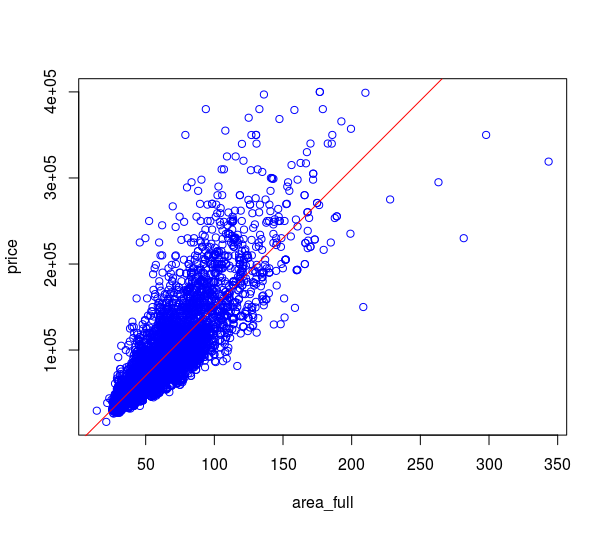
\includegraphics[scale=0.9]{price_area_model.png} 
  \caption{Зависимость цены от площади}
  \label{fig:experiment:price_area_model}
\end{figure}

Построим множественную модель регрессии с учетом всех приведенных выше параметров.

Данные характеристики показывают нам, что такие параметры как
общая площадь, жилая площадь, этаж, тип дома, год постройки, качество ремонта, район города являются значимыми и оказывают существенное влияние на формирование
окончательной цены. Тип санузла не влияет на процесс формирования цены. Поэтому его можно исключить из модели.

Полученный коэффициент детерминации $R^2$ равен 0.79 оказался выше чем в модели парной регрессии, однако он все еще
недосточно велик чтобы точно формировать цену на объекты недвижимости. Далее модель стоимости строится
отдельно по числу комнат, так как этот параметр имеет наибольшее значение после площади объекта недвижимости и этот параметр
является дискретным.

\begin{figure}[!ht]
  \centering
  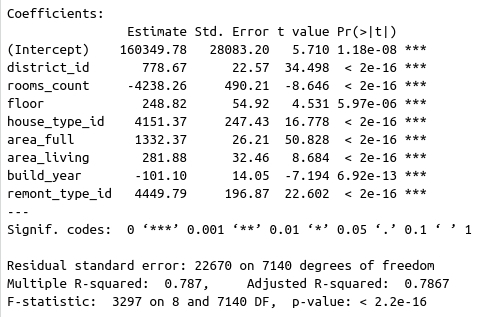
\includegraphics[scale=0.8]{multiple_model.jpg}
  \caption{Характеристики множественной модели регрессии}
  \label{fig:experiment:multiple_model}
\end{figure}

Построенные отдельно модели по числу комнат показали схожие результаты и коэффициент детерминации $R^2$ равен 0.74.
Полученная матрица корреляции представлена на рисунке~\ref{fig:experiment:corr_matrix}. Исходя из данной матрицы можно 
сделать вывод, что на конечную цену существенное влияние оказывает район города, общая площадь и жилая площадь.

\begin{figure}[!ht]
  \centering
  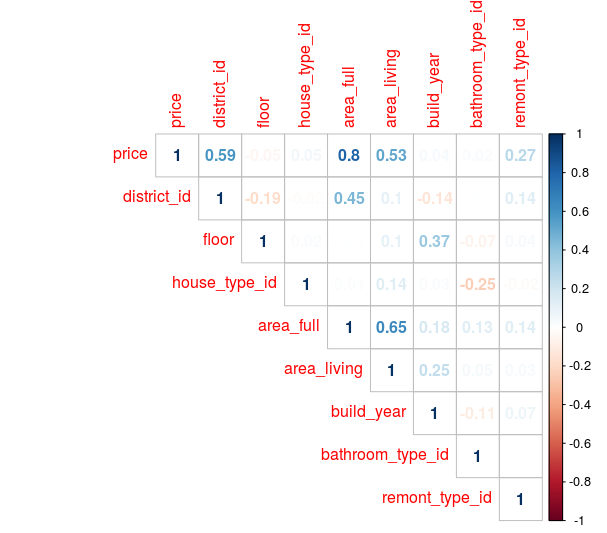
\includegraphics[scale=1]{corr_matrix.png}
  \caption{Матрица корреляции}
  \label{fig:experiment:corr_matrix}
\end{figure}

Для повышения результатов прогнозирования были построены отдельно модели по району, которые также показали схожие результаты,
однако усредненный коэффициент детерминации $R^2$ составил  0.87. Таким образом данная модель показывает лучшие результаты.

В таблице~\ref{table:experiment:regression:comparing} приведено сравнение эффективности построенных моделей.

\begin{table}[!ht]
  \caption{Сравнительная характеристика построенных моделей}
  \label{table:experiment:regression:comparing}
  \centering
    \begin{tabular}{{ 
    |>{\centering}m{0.30\textwidth}
    |  m{0.19\textwidth}
    |  m{0.19\textwidth}
    |>{\raggedright\arraybackslash}m{0.19\textwidth}|}}
  
      \hline
      Модель & {\begin{center} Коэффициент детерминации $R^2$ \end{center}} & {\begin{center} Критерий Фишера $F$ \end{center}} & {\begin{center} Остаточная стандартная ошибка $RSE$ \end{center}} \\
  
      \hline
      Парная регрессия(зависимость цены от площади) & {\begin{center}0.69\end{center}} & {\begin{center}16660\end{center}} & {\begin{center}26900\end{center}}\\
  
      \hline
      Множественная модель & {\begin{center}0.79\end{center}} & {\begin{center}2930\end{center}} & {\begin{center}22670\end{center}}\\
      
      \hline
      Отдельные модели по числу комнат & {\begin{center}0.74\end{center}} & {\begin{center}666\end{center}} & {\begin{center}10990\end{center}}\\
  
      \hline
      Отдельные модели по району & {\begin{center}0.87\end{center}} & {\begin{center}209\end{center}} & {\begin{center}8604\end{center}}\\
  
    \hline
    \end{tabular}
  \end{table}

На рисунке~\ref{fig:experiment:comparing_results} приведено сравнение прогнозируемой цены на недвижимиость
с фактической. Можно видеть, что полученная модель позволяет достаточно точно прогнозировать цену на объект недвижимости.
Исходя из этого можно сделать вывод, что предложенная модель оказалась в целом эффективной и может быть
использована для прогнозирования цены, однако результаты зависят от района продажи квартиры.

\begin{figure}[!ht]
  \centering
  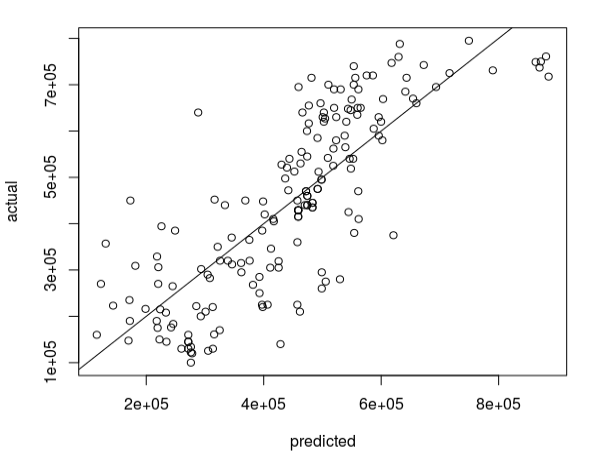
\includegraphics[scale=0.8]{comparing_results.png}
  \caption{Сравнение прогнозируемой цены с фактической}
  \label{fig:experiment:comparing_results}
\end{figure}
